\documentclass[../main.tex]{subfiles}
\begin{document}
\chapter{Modelo teórico}
toda la formulación matemática

\subsubsection{QD de dos niveles}
\begin{equation}
	H_\text{2-QD} = \omega_\sigma \sigma^\dagger \sigma
\end{equation}
donde $\omega_\sigma$ es la frecuencia de banda prohibida, o en inglés band-gap; $\sigma = \ket{v}\bra{c}$  $(\sigma^\dagger)$ es el operador aniquilación (creación) de Pauli para el QD.

\section{Sistemas Hamiltonianos de Cavidades}
\subsubsection{Cavidad fotónica}
Si se asume que tiene simetría circular y la cavidad es bimodal
\begin{equation}\label{eq:H_cav}
	H_\text{cav} = \omega_a a^\dagger a + g_a (a^\dagger \sigma_{01} + a \sigma_{10}) + \omega_b b^\dagger b + g_b (b^\dagger \sigma_{02} + b \sigma_{20}),
\end{equation}
donde $a^\dagger (b^\dagger)$ el es operador creación de fotón por polarización derecha (izquierda) dentro de la cavidad, $\omega_a (\omega_b)$ es la frecuencia del modo, y $g_a(g_b)$ es la intensidad de interacción con el estado excitón con misma polarización.

\subsubsection{Cavidad acústica}
El Hamiltoniano de la cavidad acústica tiene en cuenta el modo de energía de los fonónes individualmente
\begin{equation}\label{eq:H_cav-ph}
	H_\text{cav-ph} = \omega_b b^\dagger b
\end{equation}
donde $b^\dagger (b)$ es el operador creación (aniquilación) del modo fonónico con frecuencia de resonancia $\omega_b$

\section{Sistemas Hamiltonianos de Bombeos coherentes}
Un bombeo coherente se caracteriza por tener frecuencia y polarización bien definidas. El bombeo láser puede ser pulsado o continuo, lo que los diferencia es que su intensidad, o impulso, depende del tiempo o no. Por lo tanto, la cavidad puede ser bombeada pulsada o continuamente.

El impulso $\Omega_i(t)$ se define a partir de parámetros como: la amplitud del campo láser, el coeficiente de transmisión de la cavidad y el tipo de campo láser\footnote{$\Omega_i$ para un cw, en inglés continuous wave (cw), láser no depende del tiempo, es decir, es dependiente del tiempo en el caso de un bombeo pulsado.}. Si la forma de interacción del láser elegida es Gaussiana\footnote{Otra forma común es Lorentziana.}, entonces
\begin{equation}
	\Omega_i(t) = \Omega_{0i}\exp[-(t-t_c)^2/2\tau^2] (i=a,b)
\end{equation}
donde $\Omega_{0i}$ es el valor máximo de energía del pulso, $t_c$ es el tiempo del centro del pulso y $\tau$ es la anchura rms Gaussiana.

\subsubsection{Láser a una cavidad fotónica bimodal con QD de 5 niveles}
Se puede modelado por
\begin{equation}\label{eq:H_pump}
	H_\text{pump} = \Omega_a (t) (ae^{i\omega_L t} + a^\dagger e^{-i\omega_L t}) + \Omega_b (t) (be^{i\omega_L t} + b^\dagger e^{-i\omega_L t})
\end{equation}
aquí, $\omega_L$ es la frecuencia del láser y $\Omega_a(t)[\Omega_b(t)]$ describe qué tan eficiente el modo de la cavidad puede ser bombeado con polarización derecha [izquierda].

\subsubsection{Láser a una cavidad monomodal acústica con QD de 2 niveles}
\begin{equation}
	H_\text{2-láser} = \Omega(e^{i\omega_L t} \sigma + e^{-i\omega_L t} \sigma^\dagger)
\end{equation}
donde $\Omega$ es la intensidad del láser, en este caso es un cw láser; $\omega_L$ es la frecuencia del láser y 
$\sigma = \ket{v}\bra{c}$  $(\sigma^\dagger)$ es el operador aniquilación (creación) de Pauli para el QD.

\subsubsection{Láser a una cavidad monomodal acústica con QD de 5 niveles}
Para iniciar las transiciones el QD es impulsado por un láser externo que bombea los estados brillante-excitón de la siguiente forma
\begin{equation}\label{eq:5-laser}
	H_\text{láser} = \Omega_1 (e^{-i\omega_L t}\sigma_{1v} + e^{i\omega_L t}\sigma_{v1}) + \Omega_2 (e^{-i\omega_L t}\sigma_{2v} + e^{i\omega_L t}\sigma_{v2})
\end{equation}
donde $\Omega_1$ y $\Omega_2$ son las magnitudes relativas de las amplitudes y dependen de la polarización del láser \parencite{Belhadj2009}.


A continuación se ilustran las interacciones del láser continuo con el QD que causan transiciones entre diferentes estados
\begin{figure}[th]
	\centering
	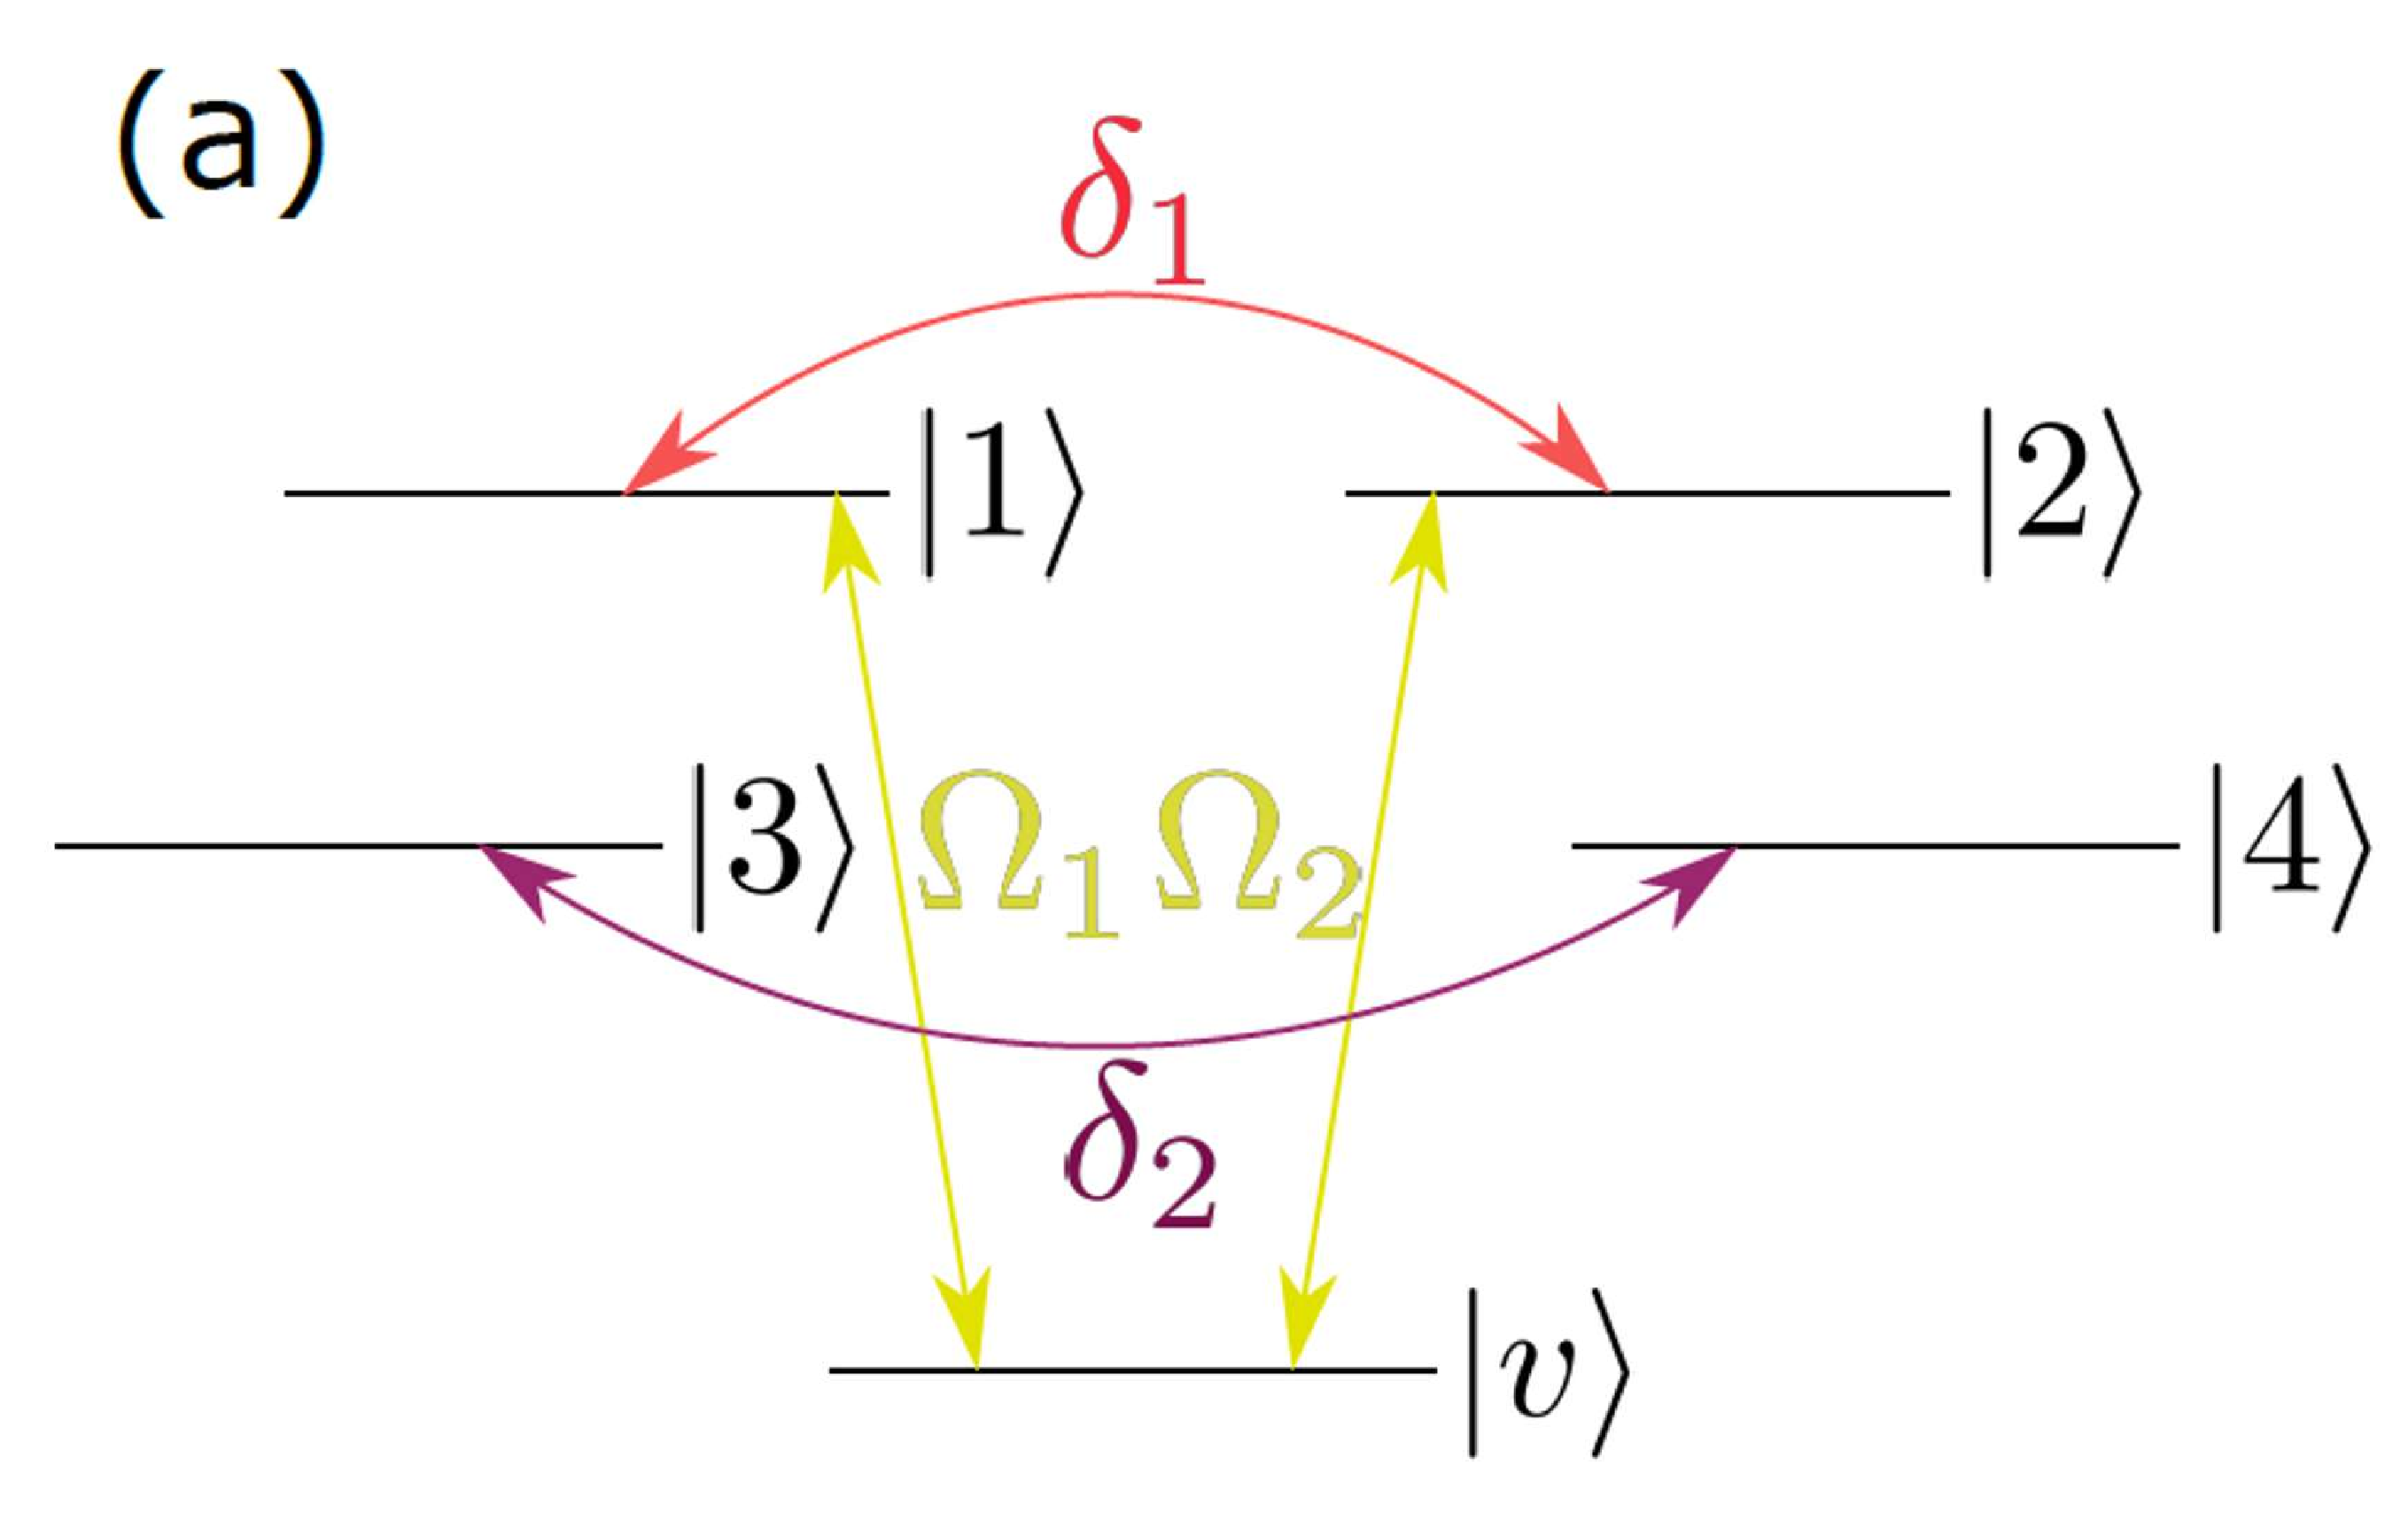
\includegraphics[width=0.35\linewidth]{img/pumpLaser}
	\caption{Interacciones que causan transiciones entre diferentes estados del QD y el láser (con las flechas bidireccionales) \parencite{Vargas2022}.}
	\label{fig:pumplaser}
\end{figure}

\subsubsection{Transformación al marco rotante}
Por medio de la transformación unitaria se remueve la dependencia temporal del Hamiltoniano del sistema completo, debido a que el láser adiciona términos que oscilan muy rápido, en el marco rotante de la frecuencia del láser 
\begin{equation}
	\tilde{H} = UHU^\dagger - \Gamma
\end{equation}
con el operador unitario
\begin{equation}
	U = \exp(i \Gamma t),\; \text{ con } \Gamma = \omega_L N_\text{ex},
\end{equation}
donde $N_\text{ex}$ es la variedad de excitación del sistema y es definida por los proyectores. Para un QD semiconductor en una cavidad acústica, donde se tienen en cuenta los estados oscuros, los proyectores son de materia, por lo tanto \parencite{Vargas2022},
\begin{equation}
	N_\text{ex} = \sigma_{11} + \sigma_{22} + \sigma_{33} + \sigma_{44}
\end{equation}
es decir, el proyector del modo fonónico ($b^\dagger b$) no se toma en cuenta.

Para una cavidad fotónica, la forma de la transformación no cambia, si se debe agregar los proyectores de los modos de dicha cavidad.

\section{Regímenes de resonancias de Stokes} \label{sec:resonancesStokes}
Un modelo a considerar donde se tengan resonancias de Stokes es en cQED\footnote{Electrodinámica cuántica de cavidades} fonónica con un QD acoplado a un modo monofonónico de una nanocavidad acústica con acoplamiento electrón-fonon $\lambda$. Un sistema punto cuántico de dos niveles con estado banda de conducción $\ket{c}$, estado banda de valencia $\ket{v}$, y frecuencia band-gap $\omega_\sigma$. El QD es impulsado por un láser óptico con frecuencia $\omega_L$ y amplitud $\Omega$. Por lo tanto, el Hamiltoniano del sistema es (con $\hbar=1$) \parencite{Bin2020}
\begin{equation}
	H = H_\text{cav-ph} + H_\text{2-QD} + H_\text{2-el-ph} + H_\text{2-láser}
\end{equation}

Las resonancias de Stokes se producen cuando un láser bombea las bandas laterales, conocidas en inglés como 'sidebands', de los fonones de orden $n$. A medida que el fonón comienza a perder energía y entra en resonancia con el punto cuántico, emite fonones con una única frecuencia permitida, es decir, la frecuencia de resonancia de la cavidad acústica. Esto se debe a que el fonón se encuentra confinado y no puede vibrar a otras frecuencias. Cuando alcanza la frecuencia de resonancia del punto cuántico, ha emitido $n$ fonones durante el proceso. Finalmente, se desexcita de nuevo al estado de valencia.

\begin{figure}[th]
	\centering
	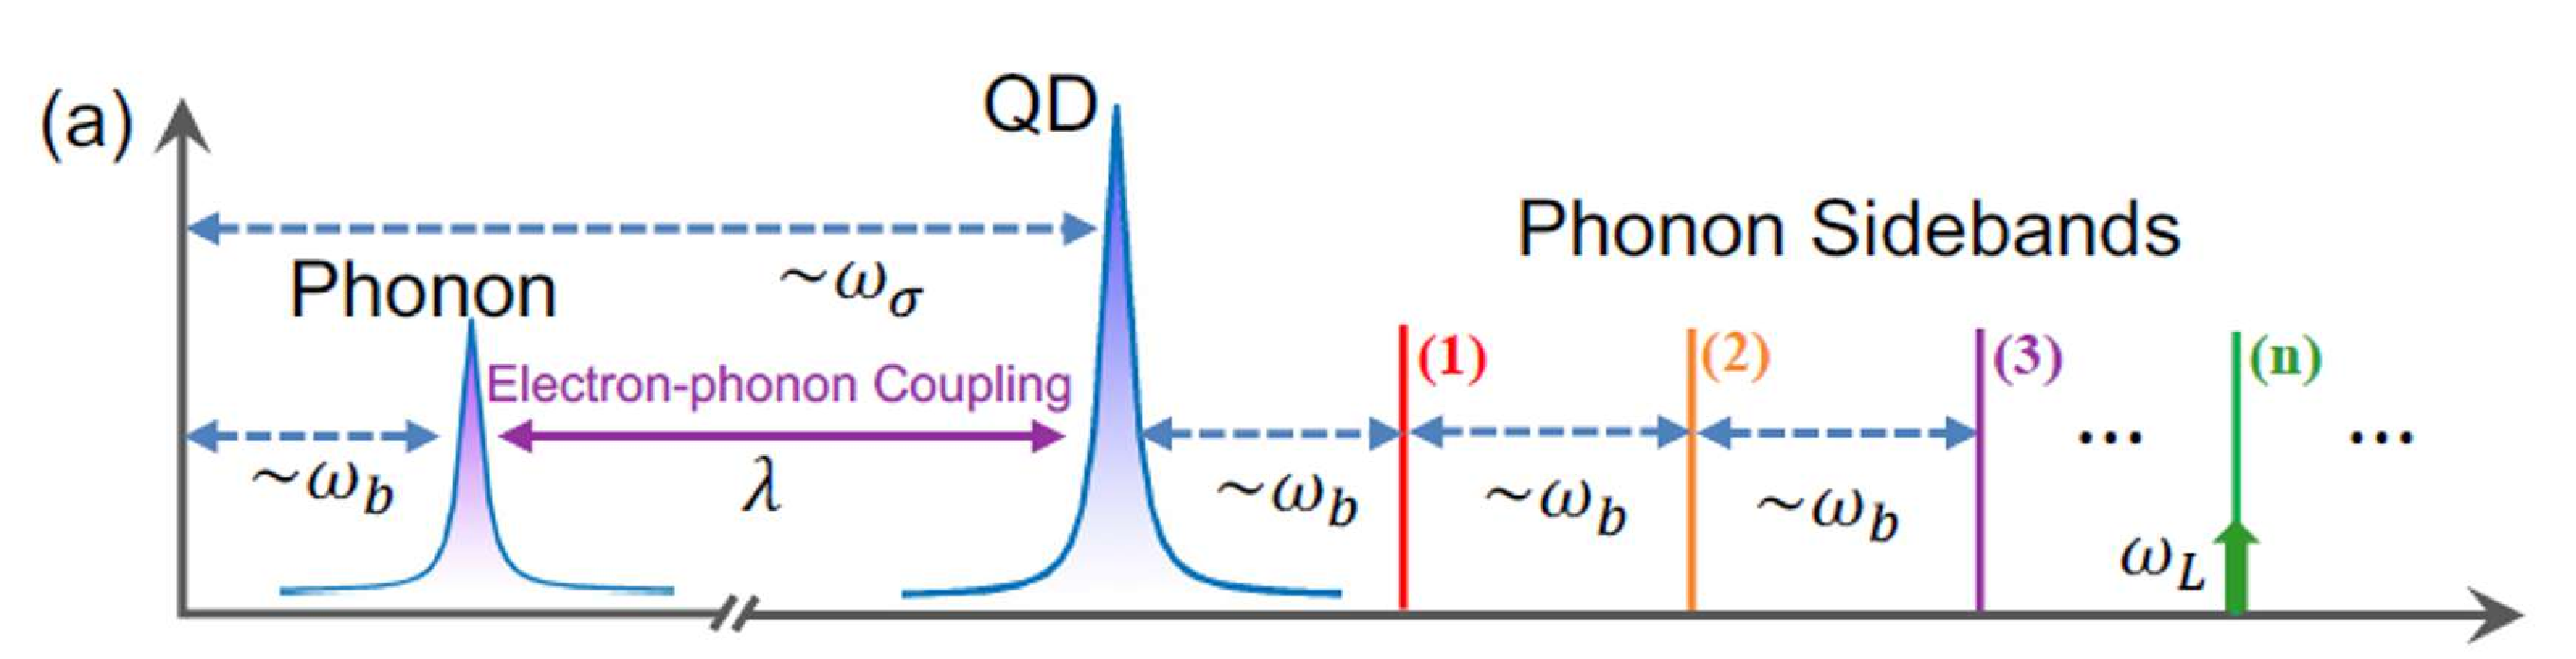
\includegraphics[width=0.85\linewidth]{img/resonancesStokes}
	\caption{Esquema del modelo y de las resonancias de Stokes en el dominio de frecuencia \parencite{Bin2020}.}
	\label{fig:resonancesstokes}
\end{figure}

\subsubsection{Régimen de acoplamiento débil electrón-fonón e impulso láser}
Parámetros $\Omega,\, \lambda \ll \omega_b$
- En este régimen los siguientes términos, debido a que no influyen significativamente en la estructura de la energía del sistema, pueden ser ignorados:- Acoplamiento electrón-fonón- Impulso laser
- En este régimen los estados propios del sistema son dados por el producto de estados $\ket{n,c/v}$, (fig. \ref{fig:resonancesstokes1})
\begin{figure}[th]
	\centering
	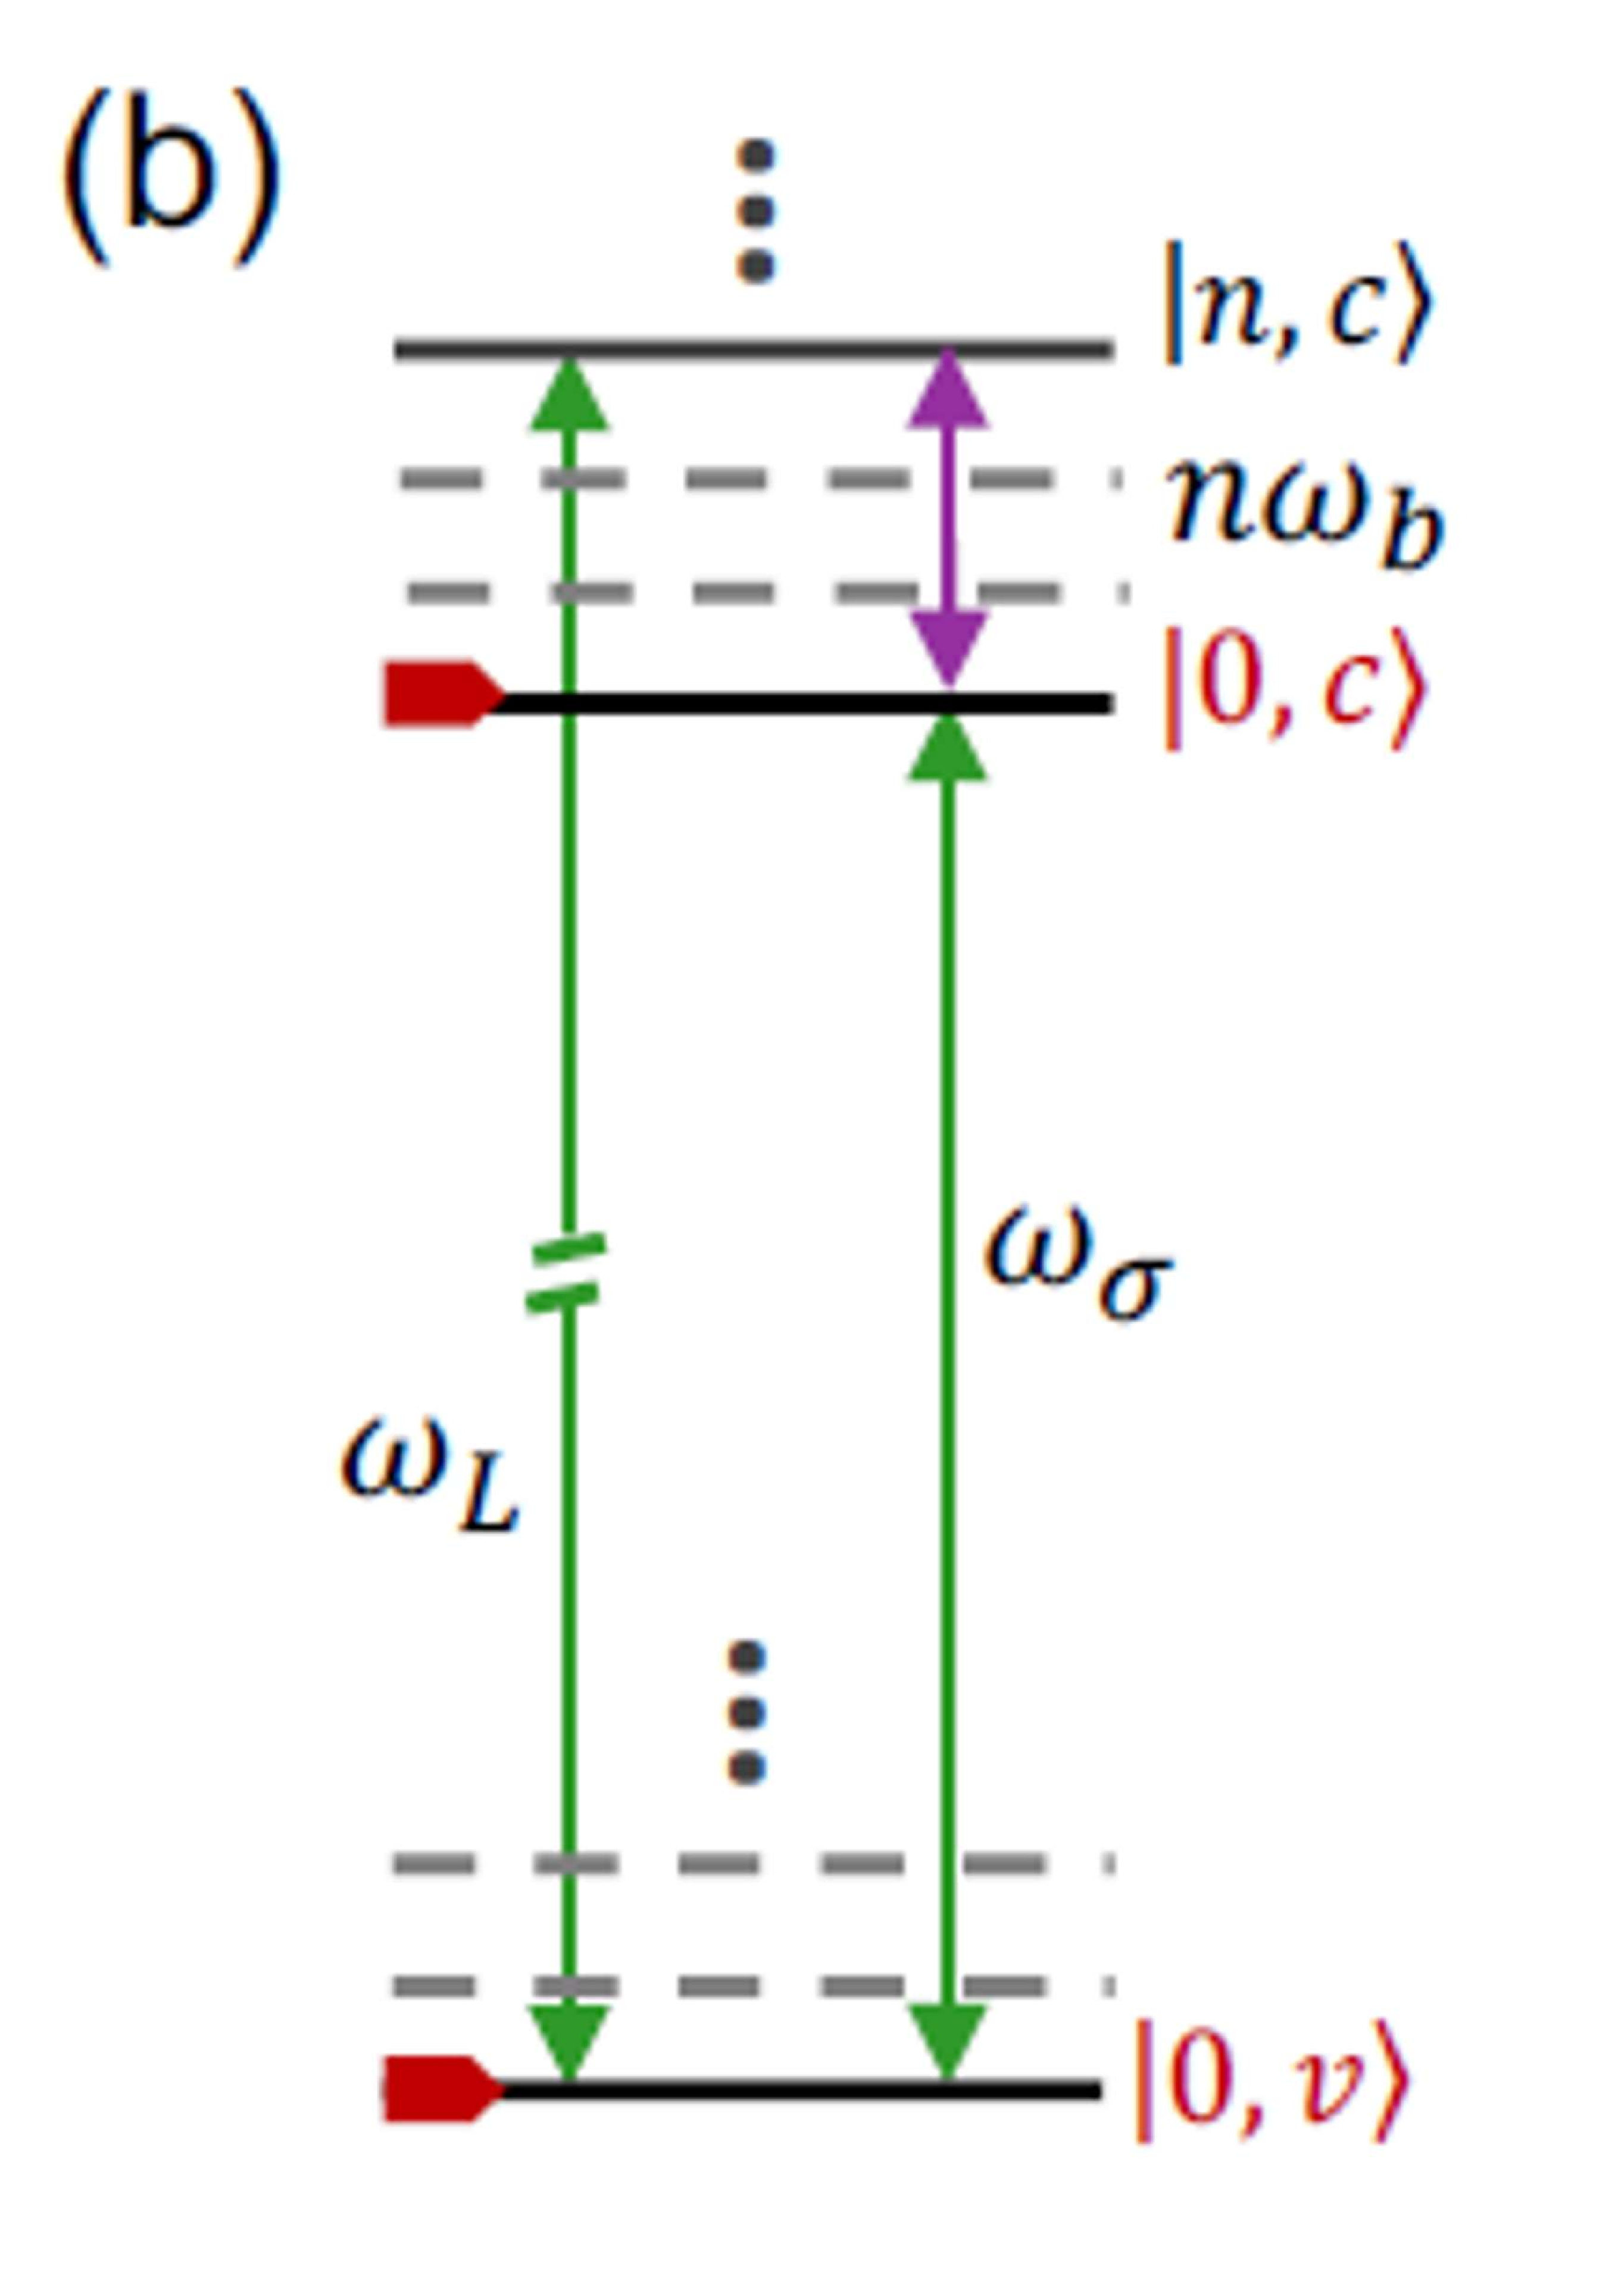
\includegraphics[width=0.25\linewidth]{img/resonancesStokes1}
	\caption{Resonancias de Stokes para el primer régimen de parámetros, a saber,  $\Omega,\, \lambda \ll \omega_b$ \parencite{Bin2020}}
	\label{fig:resonancesstokes1}
\end{figure}

La resonancia de Stokes ideal es entre estados $\ket{0,v}$, $\ket{0,c}$ y $\ket{n,c}$. Se realiza cuando el QD es impulsado a la frecuencia del sideband del fonón de $n$th-orden, es decir, $\Delta = \omega_\sigma - \omega_L = -n\omega_b$. El giro del QD es acompañado por la emisión de $n$ fonones dentro de la cavidad acústica e inducido por la interación electrón-fonón

Usando teoría de perturbaciones se encuentra que la aproximación de la tasa de transición de Stokes entre $\ket{0,v}$ y $\ket{n,c}$ conduce a oscilaciones gigante-Rabi \parencite{Bin2020}
\begin{equation}\label{eq:effRabi1}
	\Omega_\text{eff}^{(n)} = \frac{\Omega(\lambda/\omega_b)^n}{\sqrt{n!}}
\end{equation}

\subsubsection{Régimen de acoplamiento fuerte electrón fonón}
parámetros $\lambda \sim \omega_b$
El fuerte acoplamiento electrón-fonón cambia la estructura de energía, luego, conduce a condiciones de resonancia de Stokes diferentes.

Mediante una transformación desplazada $H \to DHD^\dagger$, con 
\begin{equation}
	D = \exp[(\lambda/\omega_b)\sigma^\dagger \sigma(b^\dagger - b)],
\end{equation}
el Hamiltoniano se reduce a\footnote{Con la particularidad de que este $H$ es similar al que describe un ion atrapado \parencite{Blockley1992}.}
\begin{equation}
	H = \omega_b b^\dagger b + \tilde{\omega}_\sigma \sigma^\dagger \sigma + \Omega[\sigma^\dagger e^{-i\omega_L t + \frac{\lambda}{\omega_b}(b^\dagger-b)} + \text{H.c.}],
\end{equation}
con $\tilde{\omega_a} = \omega_\sigma - \lambda^2/\omega_b$, la frecuencia de giro reescalada del QD y resonancia de Stokes $n$-fonon en $\Delta = \Delta_n(\lambda) = \lambda^2/\omega_b - n\omega_b$ (fig. \ref{fig:resonancesstokes2})

\begin{figure}[th]
	\centering
	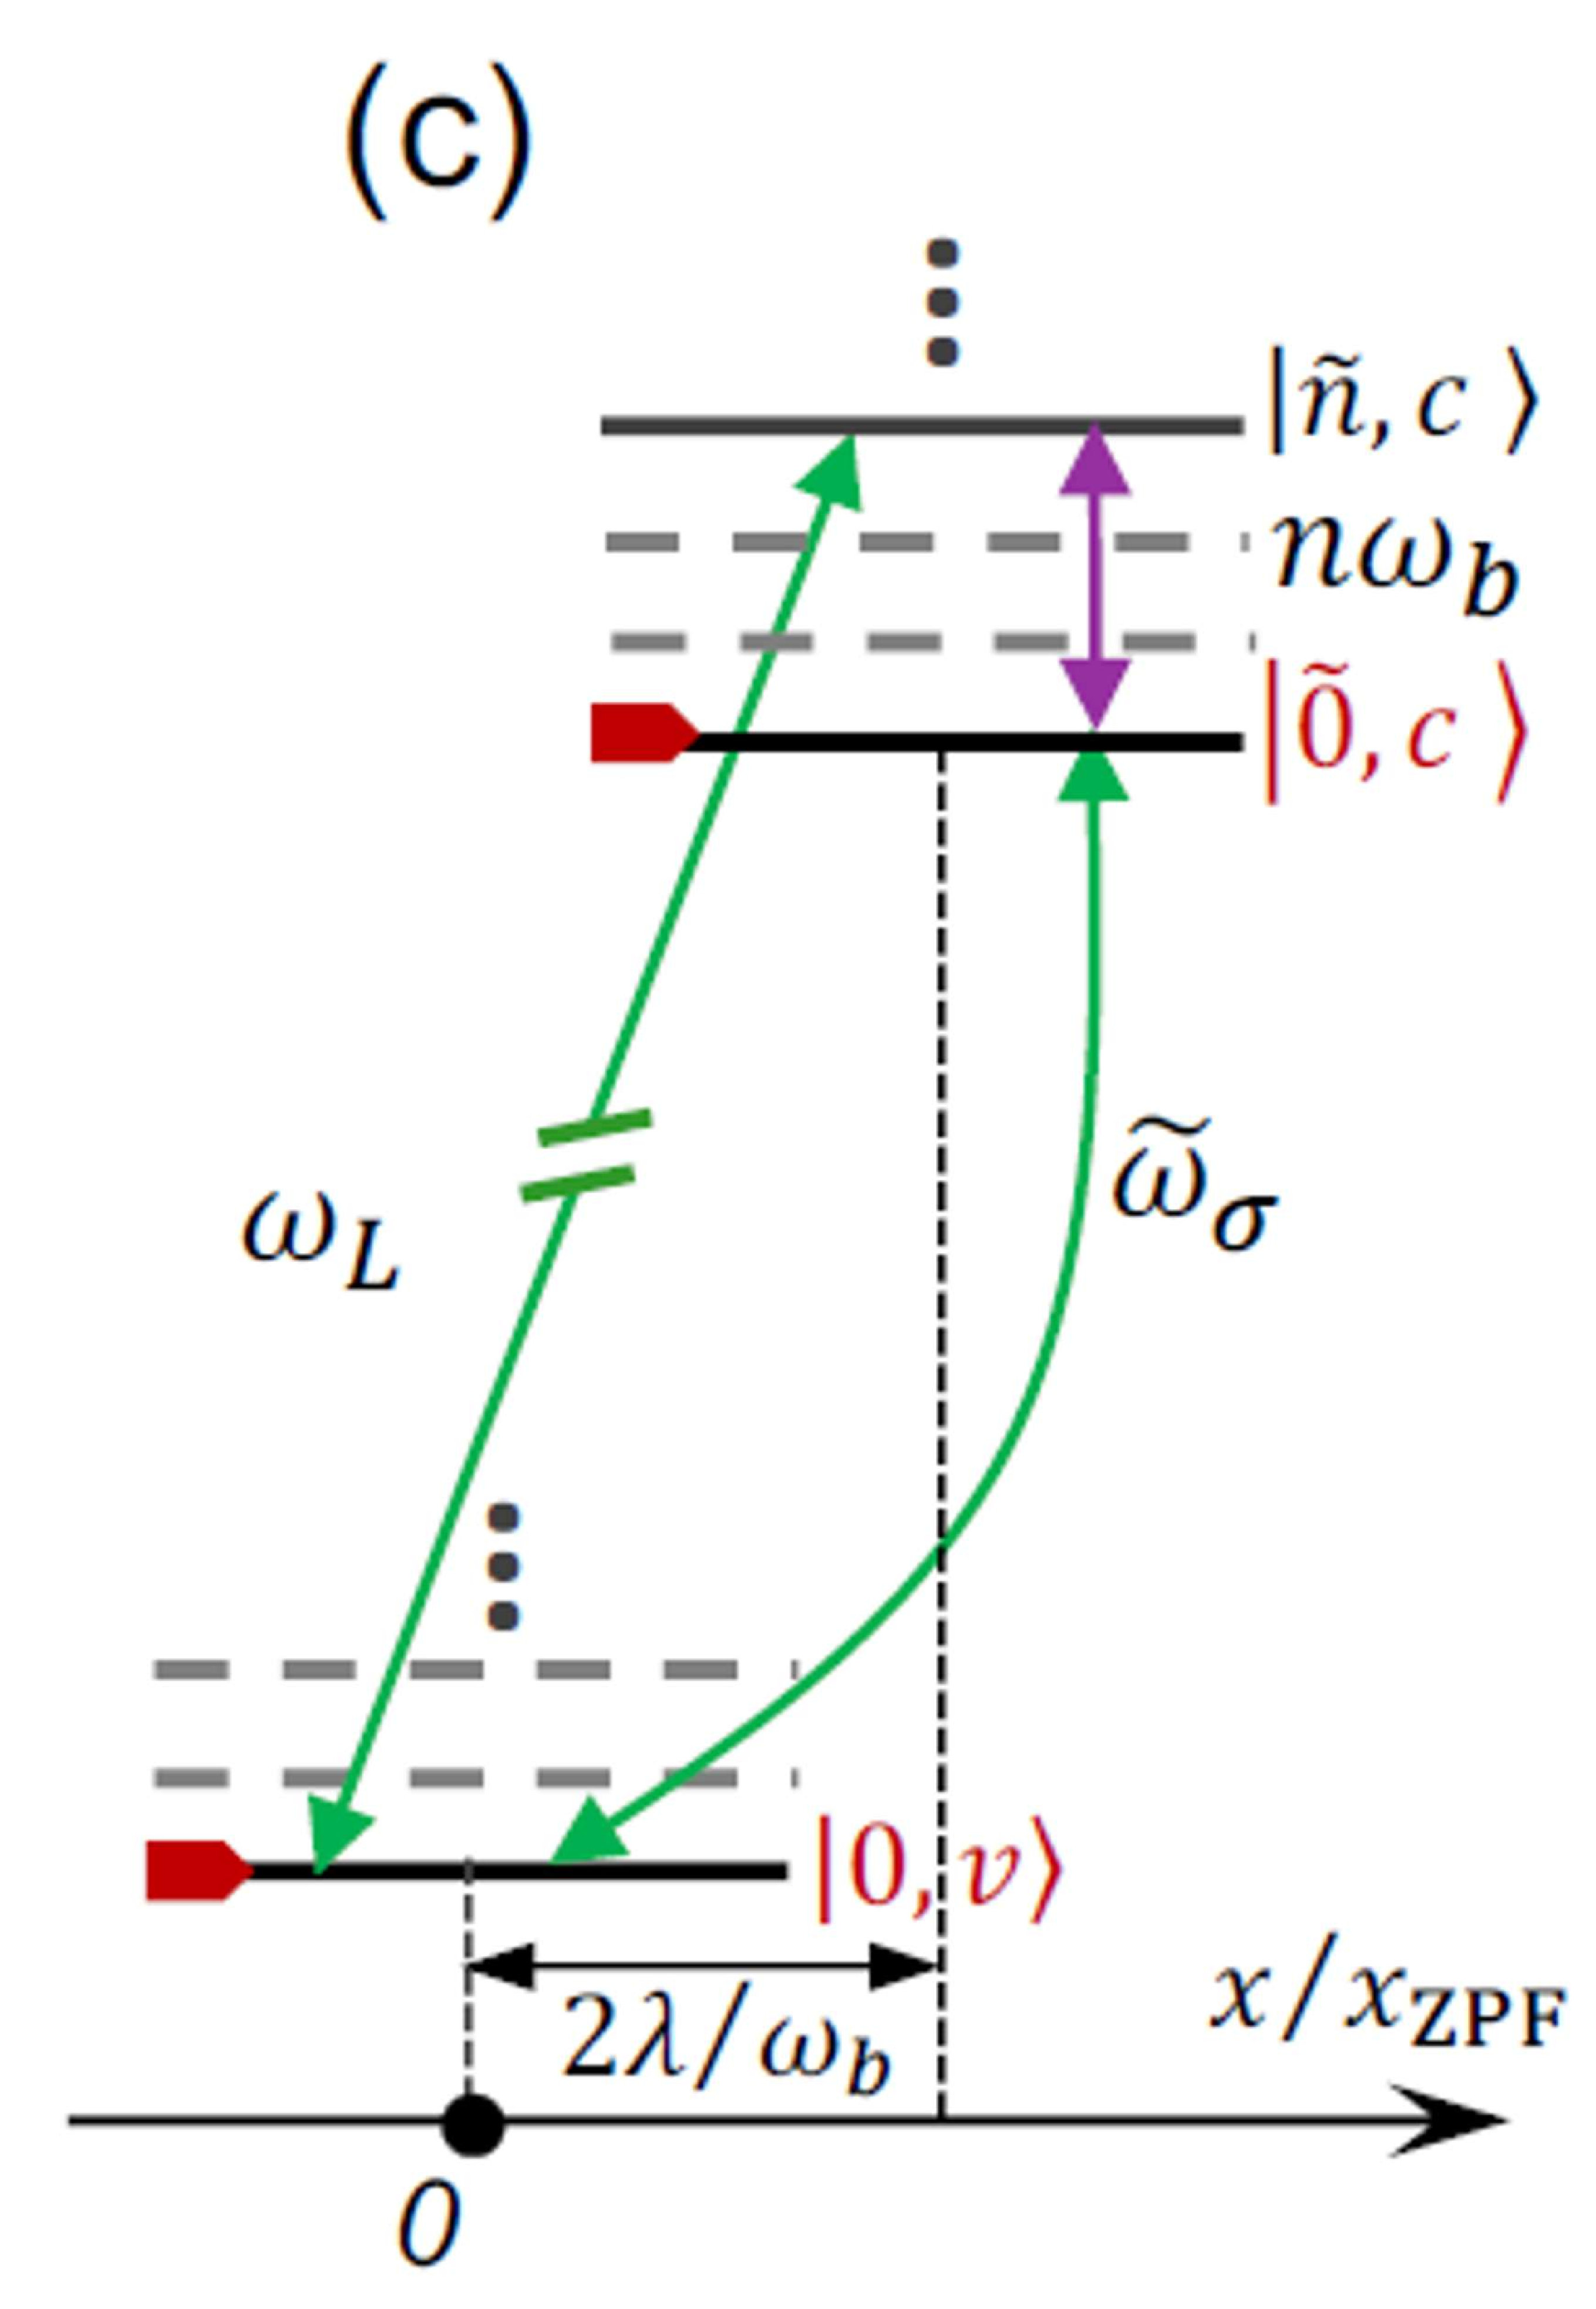
\includegraphics[width=0.25\linewidth]{img/resonancesStokes2}
	\caption{La estructura de energía cambia en el régimen de acoplamiento fuerte $\lambda \sim \omega_b$ \parencite{Bin2020}}
	\label{fig:resonancesstokes2}
\end{figure}

Ahora el producto de estados $\ket{n,c}$ es reemplazado por el estado desplazado $\ket{\tilde{n}, c} = D\ket{n,c}$ y la tasa de transición Stokes asistida $n$-fonón se vuelve \parencite{Bin2020}
\begin{equation}\label{eq:effRabi2}
	\Omega_\text{eff}^{(n)} = \frac{\Omega e^{-\lambda^2/2\omega_b^2}(\lambda/\omega_b)^n}{\sqrt{n!}}
\end{equation}

\subsubsection{Régimen de fuerte impulso del láser}
parámetros $\Omega \sim \omega_b$
\begin{figure}[th]
	\centering
	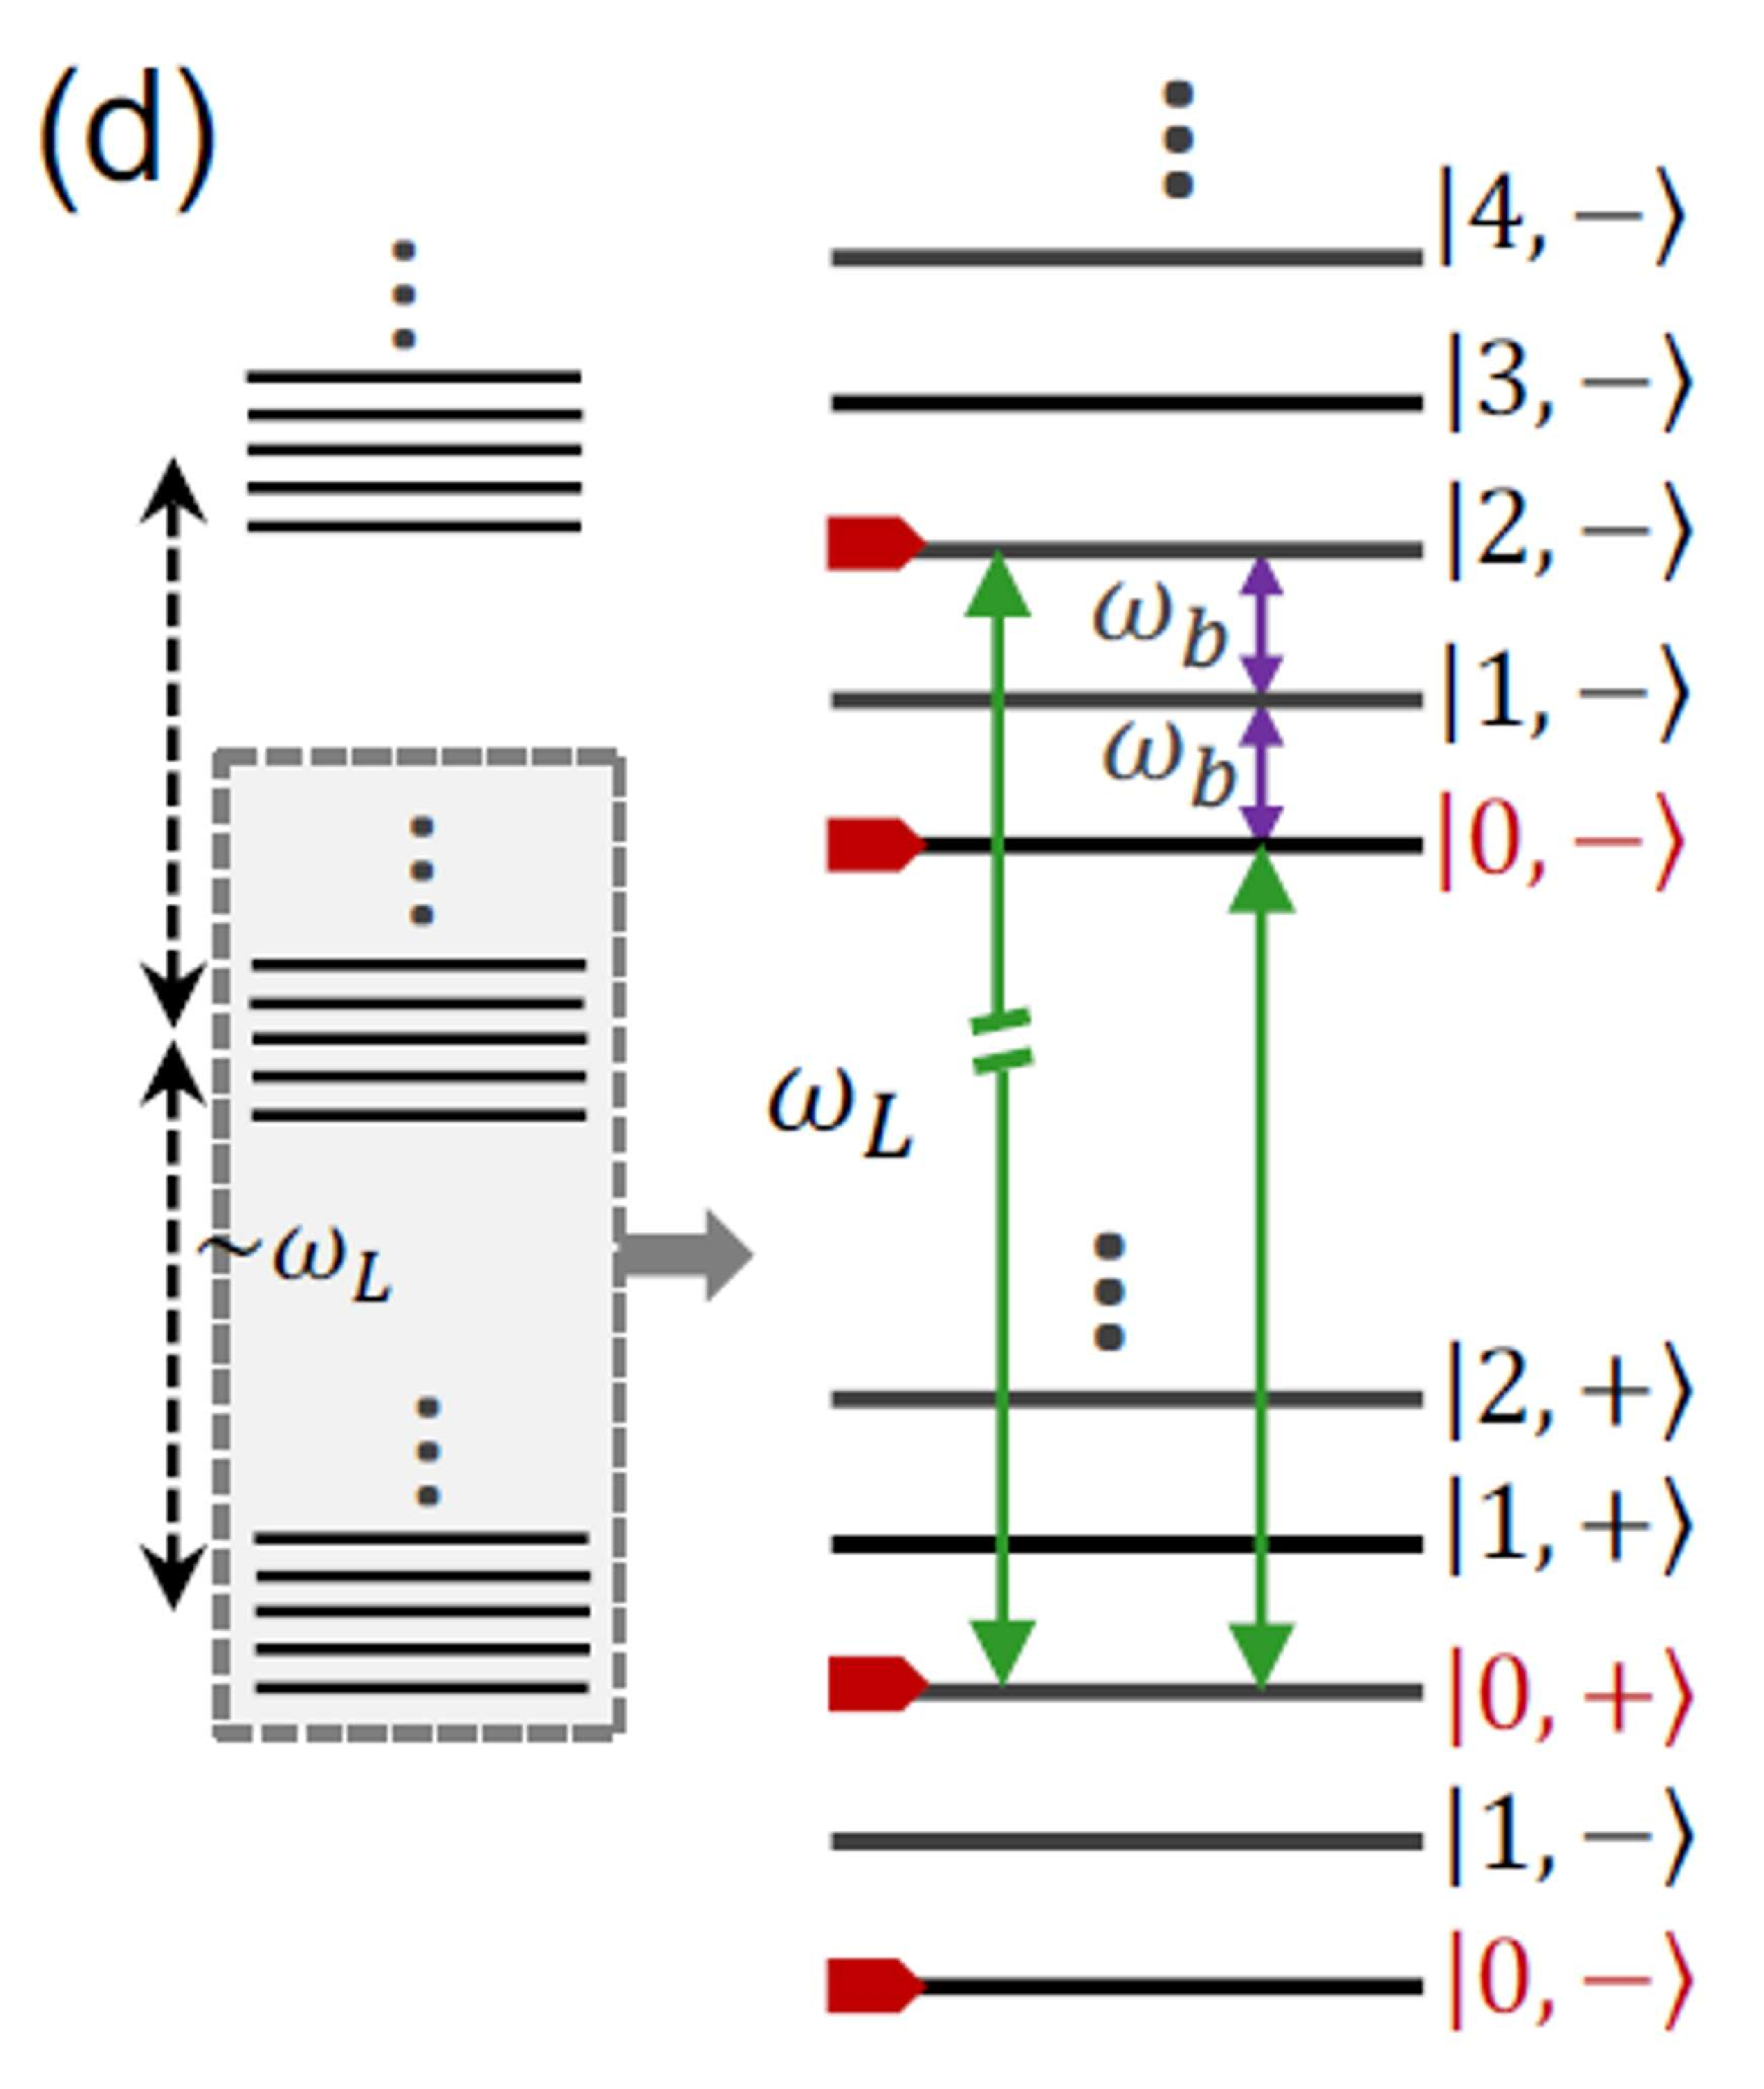
\includegraphics[width=0.3\linewidth]{img/resonancesStokes3}
	\caption{Régimen de impulso fuerte, o de Mollow, $\Omega \sim \omega_b$ \parencite{Bin2020}}
	\label{fig:resonancesstokes3}
\end{figure}
El QD se viste debido al fuerte impulso por el láser y forma una escalera de Mollow de colectores, separados por la energía del láser, donde cada colector consiste de muchos estados vestidos equidistantes $\ket{n,\pm}$\footnote{Difieren de la forma usual en sistemas cQED ópticos} con
\begin{equation}
	\ket{\pm} = c_\pm \ket{v} + c_\mp \ket{c}
\end{equation}
donde 
\begin{equation}
	c_\pm = \frac{\sqrt{2} \Omega}{(\Delta^2+4\Omega^2 \pm \Delta\sqrt{\Delta^2+4\Omega^2})^{1/2}}
\end{equation}
con valores propios correspondientes
\begin{equation}
	E_{\ket{\pm}} = \frac{\Delta}{2} \pm \frac{\sqrt{\Delta^2+4\Omega^2}}{2}
\end{equation}

Las resonancias de Stokes asistida $n$-fonón aún se realiza. Sucede cuando el láser impulsa la transición $\ket{+} \leftrightarrow \ket{-}$, en $\Delta = \Delta_n(\Omega) = -\sqrt{(n\omega_b)^2-4\Omega^2}$ y la tasa de transición correspondiente a $n$-fonón es \parencite{Bin2020}
\begin{equation}\label{eq:effRabi3}
	\Omega_\text{eff}^{(n)} = (-1)^n \Omega (\lambda/\omega_b)^n \frac{\prod_{k=1}^{n-1}(nc_-^2-k)}{(n-1)!\sqrt{n!}}
\end{equation}

En conclusión, en un amplio rango de parámetros, este sistema muestra resonancias de Stokes asociadas con la generación periódica de $n$ fonones en la cavidad acústica.

\section{Hamiltonianos de interacción}

\subsubsection{Acoplamiento electrón-fonón con un QD de dos niveles}
\begin{equation}
	H_\text{2-el-ph} = \lambda \sigma^\dagger \sigma (b^\dagger + b)
\end{equation}
donde, $\lambda$ es la intensidad de acoplamiento electrón-fonón, $\sigma = \ket{v}\bra{c}$  $(\sigma^\dagger)$ es el operador aniquilación (creación) de Pauli para el QD y $b^\dagger (b)$ es el operador creación (aniquilación) del modo fonónico.

\subsubsection{Hamiltoniano electrón-fonón con QD de 5 niveles}
Es posible acceder a los estados oscuros sin un campo magnético externo, esto debido al Hamiltoniano electrón-fonón, el cuál, tiene en cuentra el Hamiltoniano Bir-Pikus y la interacción de intercambio electrón-hueco. El Hamiltoniano Bir-Pikus está relacionado con el acoplamiento del espín del hueco al tensor de deformación del QD \parencite{Woods2004}. El Hamiltoniano electrón-phonon es
\begin{multline}\label{eq:H_el-ph}
	H_\text{el-ph} = \big\{\frac{g_{bd}}{\sqrt{2}}[(1+i)(\sigma_{13} + \sigma_{14} + (1-i)(\sigma_{23} + \sigma_{24})]\\ + g_{bb} [\sigma_{11} + \sigma_{22} + i(\sigma_{12} - \sigma_{21})] \big\} (b^\dagger + b) + \text{ H.c.}
\end{multline}
donde $g_{bb(bd)}$ son las tasas de acoplamiento a través de fonones del excitón brillante-brillante (brillante-oscuro).

El Hamiltoniano electrón-fonón es capaz de generar transiciones fonón-mediado entre excitones brillante y oscuro y entre los dos excitones brillantes \parencite{Roszak2007}. Dicha interacción, esquemáticamente, se puede visualizar en la figura \ref{fig:electron-phonon}
\begin{figure}[th]
	\centering
	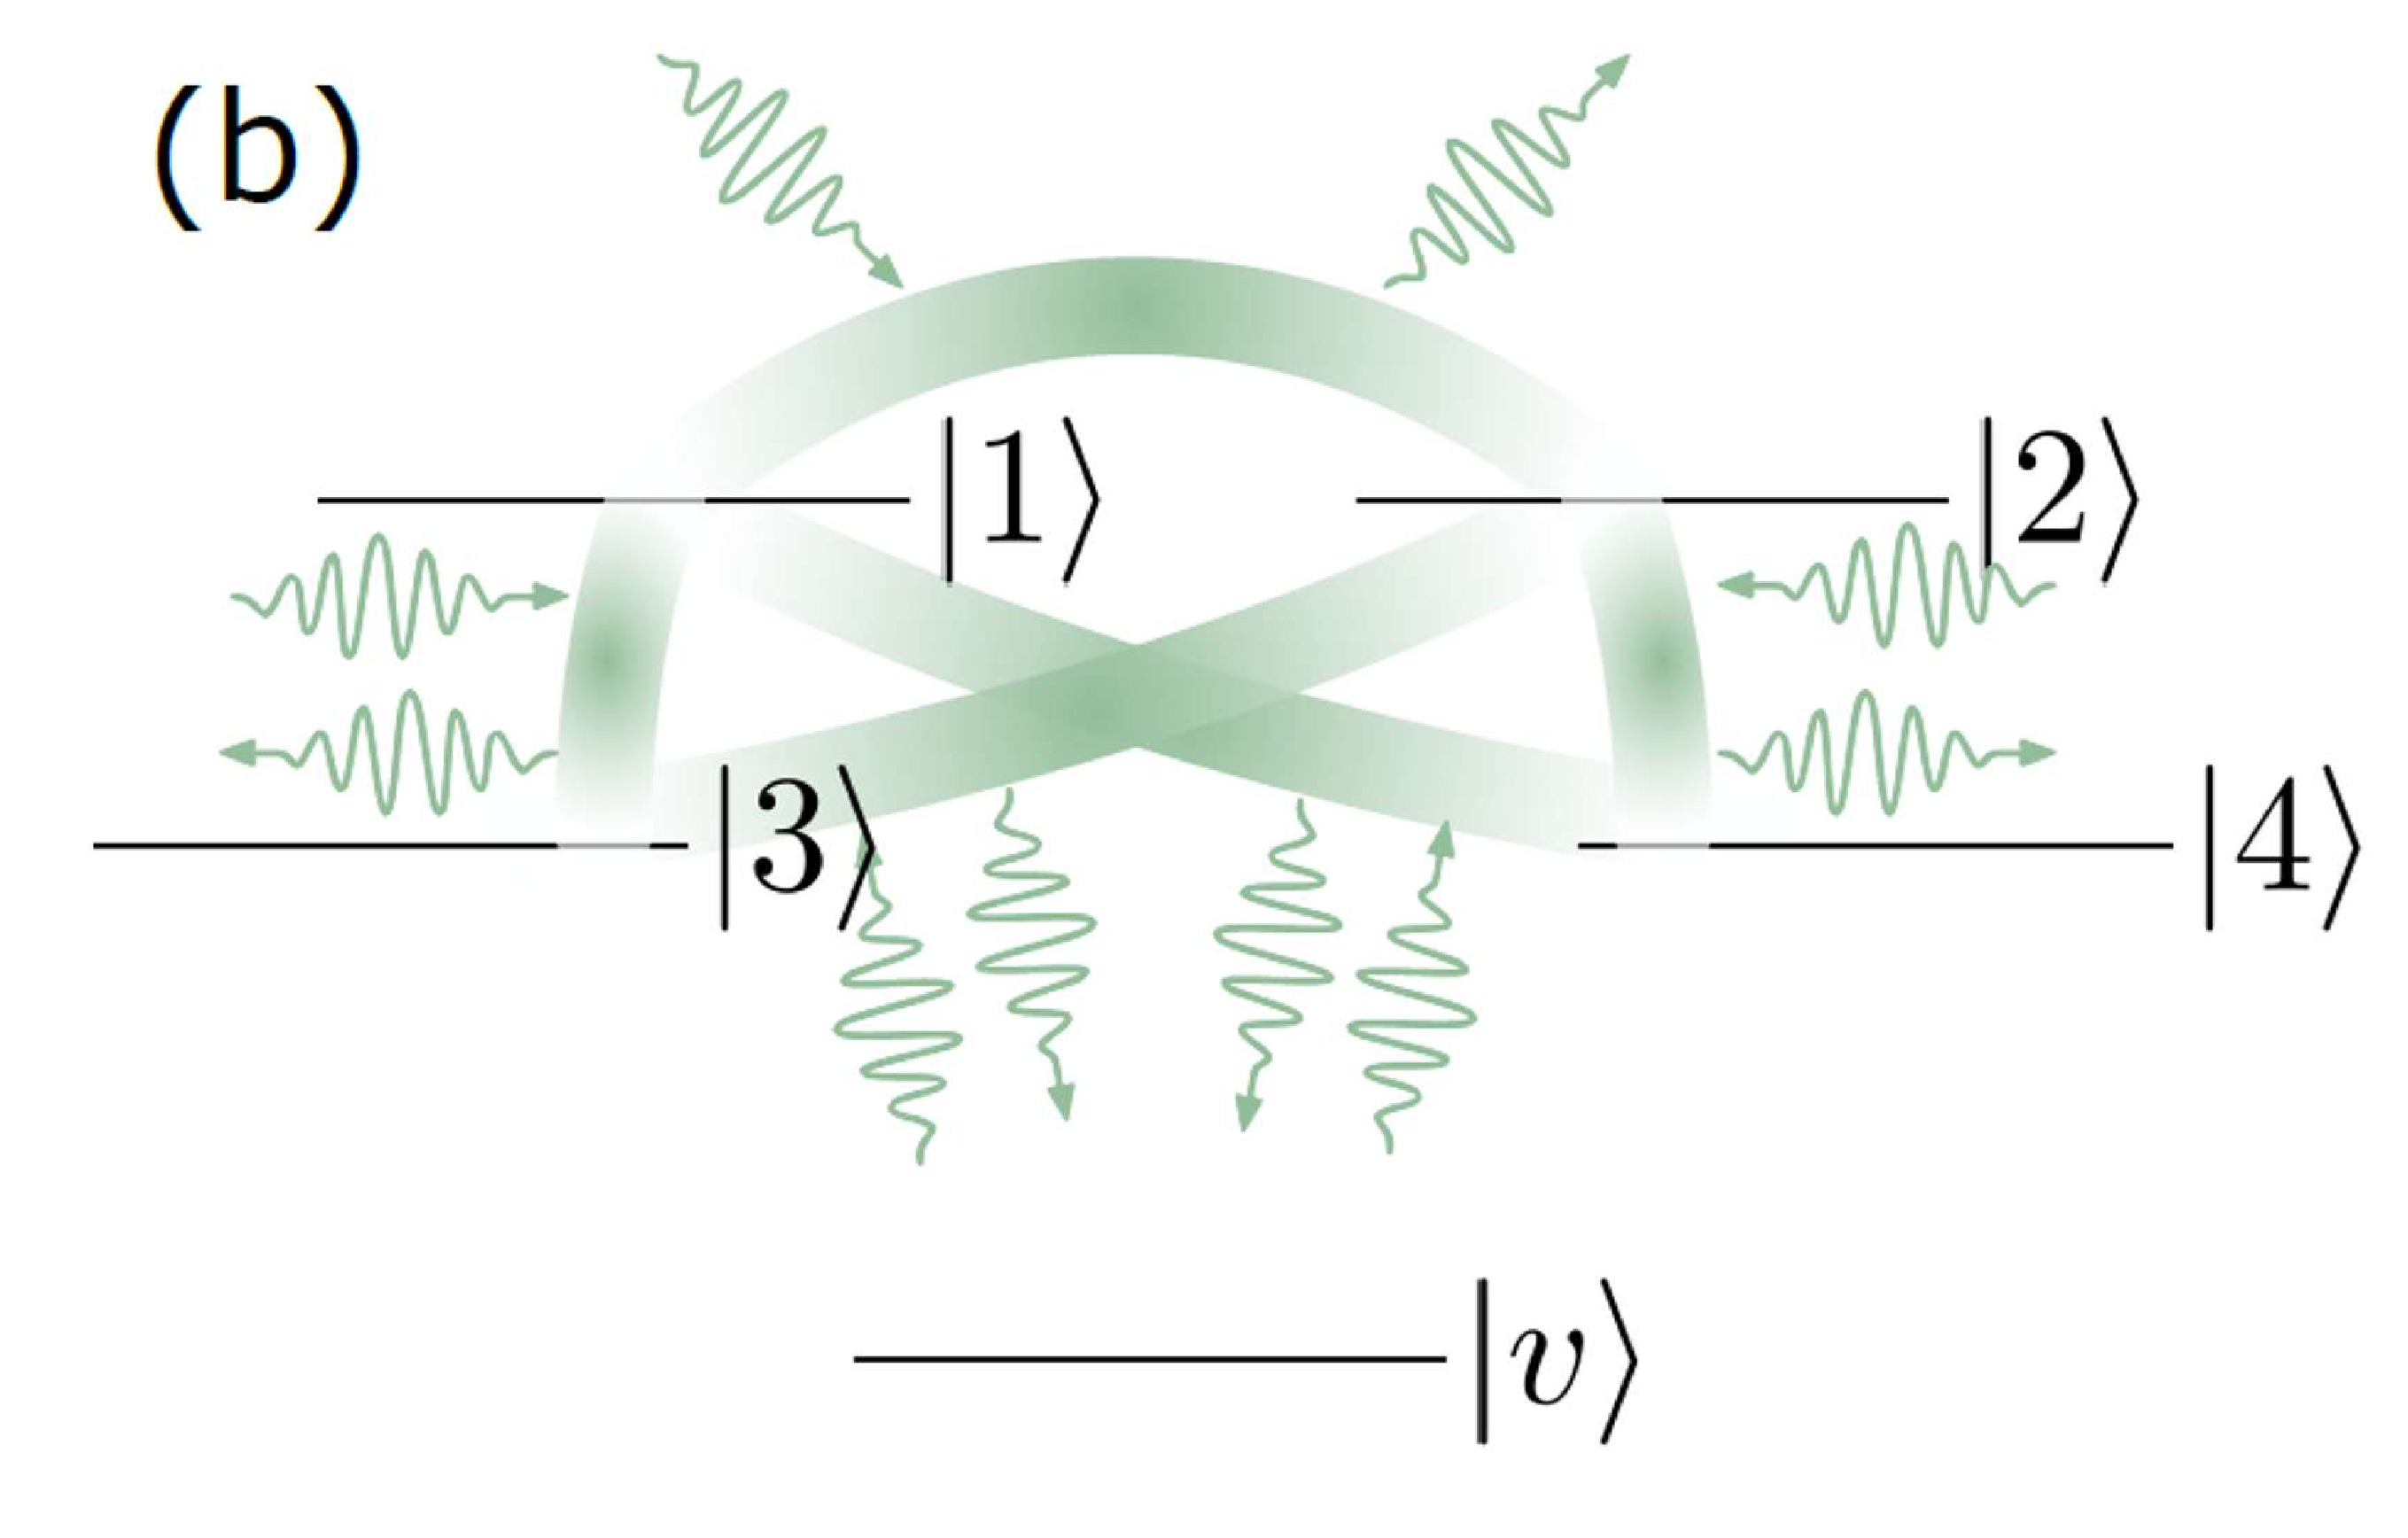
\includegraphics[width=0.35\linewidth]{img/electron-phonon}
	\caption{Muestra las interacciones representadas por $H_\text{el-ph}$ con líneas gradiente-coloreadas, que son mediadas por procesos de emisión y absorción por fonones en la cavidad acústica \parencite{Vargas2022}.}
	\label{fig:electron-phonon}
\end{figure}

\section{El operador densidad}
En el marco de la mecánica cuántica, un estado puro es ilustrado por un vector de estado $\ket{\psi}$ que es parte de un completo espacio de Hilbert. Existe una representación adicional que emplea una técnica conocida como operador de densidad, representado por $\rho$. Esta técnica, que fue propuesta en 1927 por John von Neumann, es matemáticamente idéntica a la del vector de estado pero resulta más adecuada para describir sistemas cuyos estados no se conocen completamente.

\subsubsection{Conjunto de Estados Cuánticos}
Un grupo de sistemas físicos donde cada componente se identifica por el mismo vector $\ket{\alpha_i}$ se denomina ensamble puro. En contraste, en un ensamble mixto, una fracción de los componentes se identifica por un vector $\ket{\alpha_i}$, otra fracción por un vector $\ket{\alpha_j}$, y así sucesivamente. En términos generales, un ensamble mixto puede considerarse como una combinación de ensambles puros. El operador de densidad describe el estado estadístico, ya sea puro o mixto, de un sistema cuántico.

\subsubsection{Características del operador densidad}
Un operador de densidad tiene tres propiedades principales:
\begin{subequations}
	\begin{align}
		\rho &= \rho^{\dagger}\\
		\text{Tr}(\rho) &=1\\
		\bra{\psi} \rho \ket{\psi} &\geq 0 \, \, \text{para todo} \ket{\psi},
	\end{align}
\end{subequations}
donde Tr($\rho$) es la traza\footnote{La traza se refiere a la suma de los elementos en la diagonal principal de una matriz. En este caso, esta matriz es usualmente una matriz que representa a un operador en un espacio de Hilbert finito o infinito contable.} del operador $\rho$. Las 3 propiedades aseguran que el operador es Hermítico, normalizado y semi-positivo.

El operador de densidad que corresponde a un estado cuántico está determinado por la siguiente expresión:
\begin{align}\label{eq:statePure}
	\rho = \sum_{ij} c_i c_j^* \ket{\psi_i} \bra{\psi_j}.
\end{align}

Dado que el operador de densidad se define mediante el operador de proyección, surge una propiedad de idempotencia, $\rho= \rho^2$, lo que proporciona un método directo para diferenciar los estados puros $\text{Tr}(\rho^2) =1$, de los estados mixtos donde $\text{Tr}(\rho^2) < 1$.

En el ámbito de la mecánica cuántica, la \textbf{traza} tiene varias propiedades útiles y significativas\footnote{Que se usarán para nuestra variables dinámicas.}:
\begin{enumerate}[1.]
	\item Invarianza bajo cambios de base: La traza de un operador no cambia si se realiza un cambio de base en el espacio de Hilbert. Esto la convierte en una cantidad fundamental en la teoría cuántica.
	\item La traza de un producto de operadores es invariante bajo permutaciones cíclicas: Si tienes una serie de operadores $A$, $B$, $C$, ..., la traza de su producto no cambia si permutas cíclicamente estos operadores. Es decir, Tr($ABC...$) = Tr($C...AB$) = Tr($BC...A$), etc. Esta propiedad es útil en cálculos teóricos.
	\item Cálculo de valores esperados: La traza de un operador de densidad multiplicado por un observable (otro operador) da como resultado el valor esperado de ese observable. Es decir, si $\rho$ es el operador de densidad y $A$ es un observable, entonces 
	\begin{equation}
		\text{Tr}(\rho A) = \braket{A}.
	\end{equation}
\end{enumerate}

Estas propiedades hacen de la traza una herramienta extremadamente valiosa en el análisis de sistemas cuánticos. Debido a que el operador densidad contiene toda la información físicamente relevante del sistema.

\section{Dinámica de sistemas cerrados}

La evolución temporal de un estado cuántico puro cerrado se puede obtener a partir del Hamiltoniano a través de la ecuación de Schrödinger:
\begin{equation} \label{eq:schrodinger}
	i \hbar \frac{\mathrm{d}}{\mathrm{d}t} \ket{\psi} = H \ket{\psi},
\end{equation}
donde $H$ es el Hamiltoniano del sistema, $\ket{\psi}$ es el estado cuántico y $\hbar$ es la constante de Planck reducida.

\subsubsection{Ecuación de Von Neumann}
La variación temporal del operador de densidad de un sistema cuántico aislado se representa por la ecuación maestra de \textit{Von Neumann}, la cual se deriva directamente de la ecuación de Schrödinger (\ref{eq:schrodinger}) y de la ecuación (\ref{eq:statePure})
\begin{align}\label{eq:neumann}
	i \hbar \frac{\mathrm{d} \rho}{\mathrm{d} t} = [H,\rho].
\end{align}

A pesar de que el análisis Hamiltoniano no es una configuración realista del sistema, es necesario realizarlo para comprender la física subyacente del fenómeno que se desee estudiar, por ejemplo, la producción de oscilaciones gigante-Rabi.

\section{Dinámica de sistemas abiertos}
El ambiente en el que un sistema cuántico está inmerso juega un papel crucial en la dinámica del sistema. En particular, las interacciones con el ambiente causan dos tipos de procesos: la disipación y la decoherencia. 

La \textbf{disipación} se refiere al proceso por el cual un sistema cuántico pierde energía al ambiente. Por ejemplo, un átomo que emite un fotón a su entorno está experimentando un proceso de disipación. 

Por otro lado, la \textbf{decoherencia} se refiere al proceso que destruye la coherencia cuántica, una característica esencial de la mecánica cuántica. La coherencia cuántica es la capacidad de un sistema cuántico para existir en múltiples estados a la vez (una superposición de estados). Cuando se presenta la decoherencia, el sistema evoluciona a un estado en el que ya no es posible describirlo como una superposición de múltiples estados.

Para describir con precisión la dinámica de un sistema cuántico en presencia de disipación y decoherencia, necesitamos utilizar un formalismo que vaya más allá de la ecuación de Schrödinger. Aquí es donde entran en juego la ecuación maestra y el formalismo de Lindblad\footnote{Garantiza que el operador de densidad sigue siendo válido en el transcurso del tiempo.}.

\subsubsection{Sistema cavidad bimodal-QD, de 5 niveles, bajo un campo magnético externo con inclinación}
Para obtener la dinámica del sistema se soluciona numéricamente la matriz densidad dependiente del tiempo $\rho(t)$ en la forma de Lindblad,
\begin{equation}\label{eq:masterEquationMagnetic}
	\frac{d\rho}{dt} = -i [H,\rho] + \kappa_a \mathcal{D}[a] + \kappa_b \mathcal{D}[b] + \gamma_1 \mathcal{D}[\sigma_{01}] + \gamma_2 \mathcal{D}[\sigma_{02}] + \gamma_3 \mathcal{D}[\sigma_{03}] + \gamma_4 \mathcal{D}[\sigma_{04}]
\end{equation}
donde $\mathcal{D}[L] = L\rho L^\dagger - \tfrac{1}{2}(L^\dagger L \rho + \rho L^\dagger L)$ es el superoperador Lindblad. Contiene los términos incoherentes de la matriz densidad. Se asume una aproximación Markoviana. Aquí $\kappa_a(\kappa_b)$ es la tasa de pérdida de fotón del modo de la cavidad con polarización derecha (izquierda). $\gamma_1 (\gamma_2)$ es la tasa de decaimiento del BE $\ket{1} (\ket{2})$. Se asume una tasa de decaimiento para los DEs $\gamma_3$ y $\gamma_4$.

Para solucionar la ecuación maestra se expande los operadores en una base
\begin{equation}
	\ket{\psi} = \ket{n_a}\ket{n_b}\ket{s} = \ket{n_a, n_b, s}
\end{equation}
donde $\ket{n_a} (\ket{n_b})$ es la base de Fock para el modo de la cavidad con polarización derecha (izquierda). $\ket{s}$ es el estado QD descrito antes. Manejan el truncamiento de la base de Fock de tal forma que la ocupación máxima del fotón $(\braket{a^\dagger a}, \braket{b^\dagger b})$ no cambia cuando el tamaño de la base cambie en uno. Un truncamiento más pequeño que 20 para cada polarización fue suficiente. Debido a que se usó un campo láser de baja intensidad. Se consideró el estado inicial el estado base del QD y sin fotones en la cavidad $(\ket{\psi(0)} = \ket{0,0,0})$

\subsubsection{Sistema cavidad acústica monomodal-QD, de 2 niveles con acoplamiento electrón-fonón}
Se implementa con una ecuación maestra tipo Lindblad
\begin{equation}
	\frac{d\rho}{dt} = -i[H,\rho] + \kappa \mathcal{L}[b] + \gamma \mathcal{L}[\sigma] + \gamma_\phi \mathcal{L}[\sigma^\dagger \sigma],
\end{equation}
donde
\begin{equation}
	\mathcal{L}[O] = (2O\rho O^\dagger - \rho O^\dagger O - O^\dagger O \rho)/2,
\end{equation}
$\kappa (\gamma)$ es la tasa de decaimiento de la cavidad (QD) y $\gamma_\phi$ es la tasa de decaimiento del dephasing puro del QD.

\subsubsection{Sistema cavidad acústica monomodal-QD, de 5 niveles con acoplamiento electrón-fonón}
Para estudiar la disipación se asume un acoplamiento débil al entorno, este conduce a las usuales aproximaciones Born-Markov \parencite{Breuer2007}, y se consideran cuatro canales disipativos:
\begin{enumerate}
	\item Escape de fonones de la nanocavidad acústica a una tasa $\kappa$ con un operador colapso\footnote{Un operador colapso es el que se ingresa al superoperador Disipador, ejemplo particular, $\mathcal{D}_b[\rho]$} $b$ debido al acoplamiento no deseado con los modos de fuga [55,56]
	\item Emisión espontánea de los excitones brillantes a una tasa $\gamma_b$ con los operadores colapso $\sigma_{vj}$ para $j=1,2$
	\item Emisión espontánea efectiva de los excitones oscuros (spin flip del electrón o el hueco seguido de una emisión espontánea del excitón brillante \parencite{Crooker2003}) a una tasa $\gamma_d$ con operadores colapso $\sigma_{vj}$ para $j=3,4$
	\item Desfase puro de todos los estados excitón a una tasa $\gamma_\phi$ con operadores colapso $\sigma_{jj}$ \parencite{Takagahara2002}.
\end{enumerate}

El estudio disipativo se hace bajo la ecuación Gorini-Kossakowski-Sudarshan-Lindblad, para los sistemas operador densidad
\begin{equation}\label{eq:dissipativeMasterEquation}
	\frac{d\rho}{dt} = i[\rho,H] + \kappa \mathcal{D}_b[\rho] + \gamma_b \sum_{j=1,2} \mathcal{D}_{\sigma_{vj}}[\rho] + \gamma_d \sum_{j=3,4} \mathcal{D}_{\sigma_{vj}}[\rho] + \gamma_\phi \sum_{j=1}^4 \mathcal{D}_{\sigma_{jj}}[\rho],
\end{equation}
donde
\begin{equation}
	\mathcal{D}_A[\rho] = A\rho A^\dagger - \frac{1}{2} \rho A^\dagger A - \frac{1}{2} A^\dagger A \rho,
\end{equation}
es el superopeador disipador del operador de colapso $A$.

\section{Teoría espectral}\label{sec:spectralTheory}
La interpetación de cada pico de un espectro de emisión se realiza a través de la teoría espectral del operador Liouviliano $\mathcal{L}$, el cual satisface la ecuación maestra escrita como \parencite{Manzano2018}
\begin{equation}
	\frac{d\rho}{dt} = \mathcal{L}[\rho].
\end{equation}

La solución formal de la ecuación maestra del operador Liouviliano independiente del tiempo es
\begin{equation}
	\rho(t) = \sum_k e^{\Lambda_k t} \text{Tr}[\varrho_k \rho(0)] \varrho_k
\end{equation}
donde $\Lambda_k$  son los valores propios complejos de $\mathcal{L}$ y eigenmatrices $\varrho_k$. Los $\Lambda_k$ son asociados con los picos de emisión \parencite{Vargas2018}, la ubicación del pico con $\text{Im}{(\Lambda_k)}$ y el ancho completo a mitad máxima $\text{Re}(\Lambda_k)$, las automatrices nos dan información de los estados que estan involucrados en cada transición\footnote{Se pueden estudiar sistemáticamente cuando involucren cambios en el número de excitaciones únicamente a través de procesos disipativos.}. Sin embargo, para el sistema de la sección \ref{sec:giant-Rabi} no es posible usar la teoría espectral completamente debido a la presencia del bombeo coherente al QD, sin embargo, al examinar las eigenmatrices aún muestran qué estados están involucrados en las transiciones (ver fig. \ref{fig:emissionspectrumgiant-rabi}((a) y (b)))
%
\end{document}